\chapter{\IfLanguageName{dutch}{Proof of Concept}{Proof of Concept}}%
\label{ch:PoC}

Dit deel van het onderzoek presenteert een proof of concept gericht op welk framework er gebruik zal worden om machine learning pipelines lokaal uit te voeren, dat gebruikt kan worden in de cursus ``Machine Learning Operations''.
Het doel van deze proof of concept is om de efficiëntie en bruikbaarheid van deze frameworks te onderzoeken aan de hand van een lokale opstelling met de gekozen frameworks. Hierbij zullen de uitvoeringen van het framework, alsook de resultaten en bevindingen, besproken worden.
Hierna wordt aan de hand van de resulaten een conclusie getrokken over het gekozen framework.
\section{Vereisten}

% TODO: beschrijf ook de specs van jouw pc, de software-versie, eventuele configuratie en installatie-stappen (of verwijs naar documentatie).

Voordat we kunnen beginnen met het uitwerken van de volgende Proof of Concepts, zijn bepaalde vereisten nodig. De vereisten zijn als volgt:
\begin{itemize}
    \item Python moet geïnstalleerd zijn, dit kan worden gedaan via de documentatie.
    \item De package manager ``pip''
\end{itemize}
Deze vereisten zorgen ervoor dat de volgende hoofdstukken zonder problemen werken. Als hardwarevereisten is het voldoende om te voldoen aan de minimale vereisten van de opleiding Toegepaste Informatica. De Proof of Concept zal ook geen configuratiebestanden veranderen voor de lokale opstelling; alles wordt met de standaardinstellingen uitgevoerd.
\section{Ontwikkeling van de Machine Learning pipeline}
% TODO: ik lees vaan "in dit onderdeel", "in dit deel", dat leest moeizaam

De opbouw van de Machine Learning pipeline wordt besproken, wat ervoor zal zorgen dat het duidelijk is hoe de pipeline in elkaar zit. De Machine Learning pipeline die gebruikt zal worden, is die van Labo 3 van de cursus "Machine Learning Operations".
Deze pipeline is ontworpen om aan de hand van Image Classification het verschil te kunnen herkennen tussen foto's van "Appelsienen" en "Appels", zoals besproken in de stand van zaken. Deze pipeline heeft verschillende onderdelen:

\begin{itemize}
    \item \textbf{Preprocessing:} Voor het downloaden en verwerken van de afbeeldingen.
    \item \textbf{Training:} Voor het trainen van het model.
    \item \textbf{Evaluatie:} Voor het evalueren van het moel.
\end{itemize}

De volgende hoofdstukken zullen elk van deze onderdelen toelichten en de werking ervan uitleggen, zoals weergegeven in diagram \ref{fig:Model_Flow}.
\begin{figure}[htbp]
    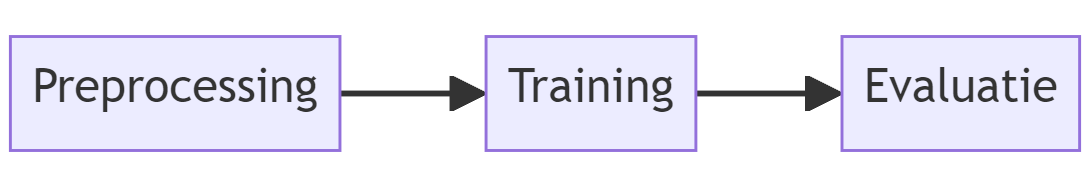
\includegraphics[width=\linewidth]{graphics/Model_Diagram.PNG}
    \caption{Model Flow}
    \label{fig:Model_Flow}
\end{figure}
\subsection{Packages}
Dit deel zal alle gebruikte packages kort uitleggen en hoe deze geïnstalleerd kunnen worden. De packages zijn grotendeels hetzelfde voor elke Proof of Concept, maar kunnen extra packages hebben in verband met het gekozen framework.
De basispackages die gebruikt zullen worden in de Proof of Concepts zijn:
\begin{itemize}
    \item \textbf{Tensorflow:} Voor het trainen en evalueren van het model, Tensorflow werkt samen met Keras hiervoor.
    \item \textbf{os:} Voor het maken van mappen voor de verschillende datasets die worden gebruikt tijdens de training en de evaluatie van het model.
    \item \textbf{Requests:} Voor het maken van HTTP-verzoeken naar de links van de afbeeldingen om deze dan te kunnen downloaden.
    \item \textbf{Keras:} Voor het maken van het model doormiddel van verschillende lagen.
    \item \textbf{MLFlow:} Voor het bijhouden van alle resultaten van het model, trainingsprocess en de evaluatie.
\end{itemize}

In de github van deze Proof of Concept zal voor elk framework een bestand genaamd ``requirements\_framework.txt'' te vinden zijn, waarbij ``framework'' de naam is van het gebruikte framework. Dit bestand kan samen met ``pip'' gebruikt worden om alle packages te installeren met het volgende commando:

\begin{minted}[frame=lines,breaklines,linenos]{bash}
    pip install -r "requirements.txt"
\end{minted}
\section{Virtuele omgeving}

De volgende hoofdstukken zullen gebruikmaken van verschillende frameworks. Deze frameworks hebben allemaal de mogelijkheid om lokaal een Machine Learning pipeline uit te voeren en voldoen ook aan alle nodige criteria van het requirementsanalyse.
Voor elk framework dat gebruikt zal worden, wordt er een virtuele omgeving opgesteld. Dit zorgt ervoor dat er geen conflicten zijn tussen de verschillende versies van de libraries.

\subsection{Preprocessing}
Het Preprocessing gedeelte van de pipeline bereidt de data voor zodat het model getraind kan worden. Dit omvat het laden en transformeren van de afbeeldingen, zodat deze afbeeldingen gebruikt kunnen worden als invoer voor het trainen van het model. In dit Proof of Concept wordt er gebruikgemaakt van Tensorflow's ImageDataGenerator om afbeeldingen in te laden, te normaliseren en te voorzien van labels gebaseerd op de mapstructuur. Na het inladen van de afbeeldingen en het klaarmaken ervan voor het trainen van het model, worden de afbeeldingen gesplitst in trainings-, validatie- en testsets. In elke van deze sets worden de juiste labels voorzien.
\subsection{Training}
Het Training gedeelte gaat daadwerkelijk een Machine Learning-model trainen. Deze Proof of Concept zal gebruikmaken van een Convolutional Neural Network (CNN) met behulp van Keras. Dit model bevat verschillende lagen en parameters. Er wordt gebruikgemaakt van een sequentieel model van Keras, wat betekent dat alle lagen achtereenvolgens worden uitgevoerd. De volgorde en de lagen die gebruikt worden voor dit Proof of Concept zijn als volgt:
\begin{itemize}
    \item Convolutionele laag (Conv2D)
    \item Activatielaag (Activation)
    \item Flatten-laag
    \item Dense-laag
\end{itemize}
\subsection{Evaluatie}
Het evaluatiegedeelte zal het model evalueren dat we hiervoor hebben getraind. Alle resultaten hiervan worden bijgehouden met MLFlow. De resultaten bevatten:
\begin{itemize}
    \item Parameters van het model
    \item systeemeigenschappen en performance
    \item Accuracy van het model en de evaluatie
\end{itemize}

\section{MLflow}
Elk van deze Proof of Concepts bevat MLflow, zoals besproken in de stand van zaken heeft deze framework veel functionaliteiten. Voor deze Proof of Concepts gaan we vooral de parameters van het model, de resultaten van de training en de resultaten van de evaluatie bijhouden. Dit wordt Experiment Tracking genoemd en stelt ons in staat om experimenten bij te houden.
\subsection{Installatie}
Om MLflow te gebruiken, moet het eerst geïnstalleerd en geïmporteerd worden. Hieronder staat een codevoorbeeld van hoe dit te doen:
Installeren met ``pip'':
\begin{minted}[frame=lines,breaklines, linenos]{bash}
    pip install MLFlow
\end{minted}
Importeren in een python-script of notebook:
\begin{minted}[frame=lines,breaklines, linenos]{python}
    import mlflow
    import mlflow.keras
\end{minted}

Nadat MLflow is geïmporteerd, moeten we alle parameters in de code aanpassen, zodat deze de resultaten naar de juiste server stuurt en de juiste resultaten bijhoudt. De parameters die we moeten aanpassen zijn als volgt:
\begin{itemize}
    \item Parameter Logging: Het commando hiervoor is ``mflow().log\_param''. Dit houdt alle parameters bij van het model, zoals het aantal epochs of de batchgrootte.
    \item Metric Logging: Tijdens het trainen van het model zal MLflow belangerijke resulaten bijhouden, zoals de nauwkeurigheid en het verlies van het model. Dit word aan de hand van ``mlflow.log\_metric()'' bijgehouden. Deze metrics worden voor elke epoch van het trainingsproces bijgehouden om het verloop van de training te analyseren.
\end{itemize}
Als MLflow geinstalleerd is en alle parameters correct zijn ingesteld, kan de lokale server worden opgestart met het volgende commando:
\begin{minted}[frame=lines,breaklines, linenos]{bash}
    mlflow server --host 127.0.0.1 --port 8080
\end{minted}
Dit commando heeft de volgende parameters:
\begin{itemize}
    \item \textbf{--host:} voor het instellen van het ip addres voor de lokale server.
    \item \textbf{--port:} voor het instellen van de poort van de lokale server.
\end{itemize}
Nadat de server is opgestart kan naar het ingestelde adres worden genavigeerd om het dashboard te zien.
\subsection{Dashboard}
Het dashboard van MLflow toont de resulaten van alle pipelines weer, figuur \ref{fig:mlflow_dashboard} toont het dashboard weer.
\begin{figure}[htbp]
    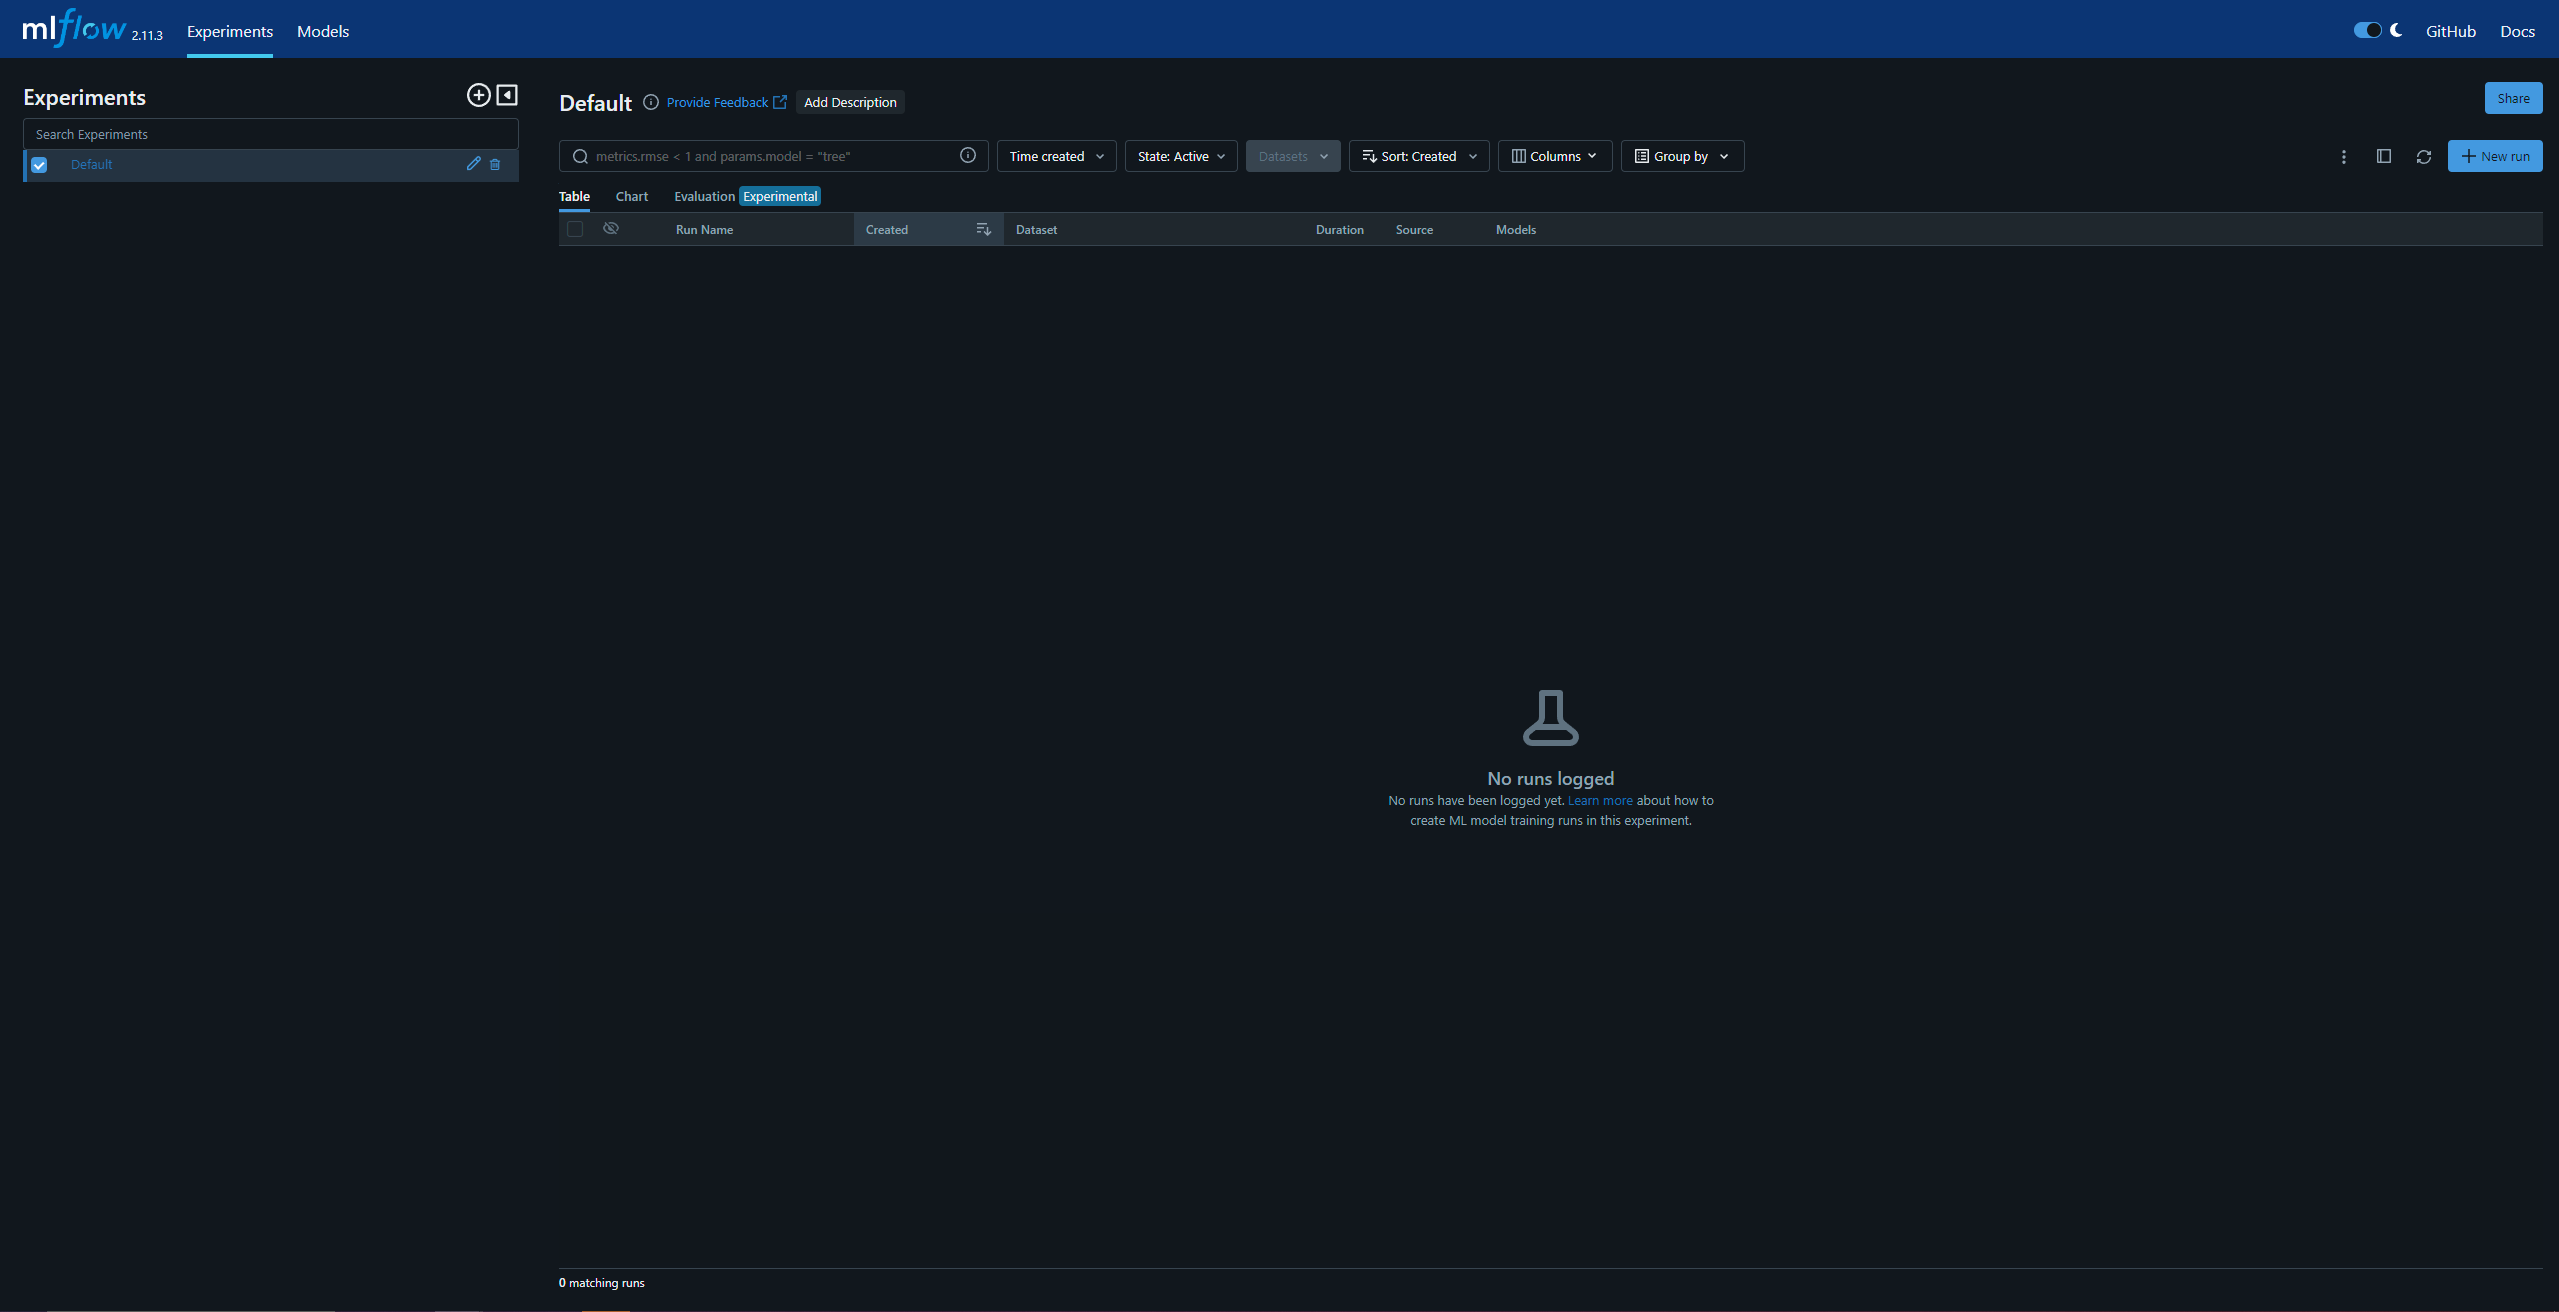
\includegraphics[width=\linewidth]{graphics/mlflow_dashboard.PNG}
    \caption{MLflow Dashboard}
    \label{fig:mlflow_dashboard}
\end{figure}

\section{Prefect}
Dit deel zal het Proof of Concept uitleggen waarbij Prefect wordt gebruikt in combinatie met MLFlow voor het lokaal uitvoeren van Machine Learning pipelines. Hierbij worden alle aanpassingen in de code van het framework vergeleken met de originele code van Labo 3 van de cursus ``Machine Learning Operations''
\subsection{Installatie}
De installatie van Prefect gebeurt met de package manager ``pip''. Via de terminal kan je met het volgende commando Prefect installeren, dit zal alle nodige libraries installeren voor deze Proof of Concept:
\begin{minted}[frame=lines,breaklines,linenos]{bash}
    pip install -r "requirements.txt"
\end{minted}

Om alleen Prefect te installeren kan dit met het volgende ``pip'' commando:
\begin{minted}[frame=lines,breaklines,linenos]{bash}
    pip install prefect
\end{minted}

\subsection{Lokale Server}
Prefect heeft de mogelijkheid om Machine Learning pipelines lokaal uit te voeren, dit gebeurt met behulp van een lokale server. Deze server kan worden opgestart met het commando:
\begin{minted}[frame=lines,breaklines,linenos]{bash}
    prefect server start
\end{minted}

Na het uitvoeren van het startcommando zou het resultaat van figuur \ref{fig:Prefect_server} te zien moeten zijn.
\begin{figure}[htbp]
    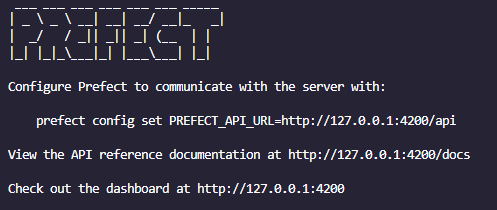
\includegraphics[width=\linewidth]{graphics/Prefect_server.PNG}
    \caption{Prefect Server Command}
    \label{fig:Prefect_server}
\end{figure}
Nu de server is opgestart, moet de code nog communiceren met de Prefect webinterface.
Zoals figuur \ref{fig:Prefect_server} aantoont, wordt dit gedaan aan de hand van een commando dat gebruikmaakt van een lokale API:
\begin{minted}[frame=lines,breaklines,linenos]{bash}
    prefect config set PREFECT_API_URL=http://127.0.0.1:4200/api
\end{minted}
Nu de server is opgestart en verbonden is met de lokale omgeving, kan via de ingestelde link het Prefect dashboard worden bezocht.
\subsection{Dashboard}
Het dashboard van Prefect is een omgeving waar alle pipeline flows worden beheerd. Figuur \ref{fig:Prefect_Dashboard} toont aan hoe dat het Prefect dashboard eruit ziet.
\begin{figure}[htbp]
    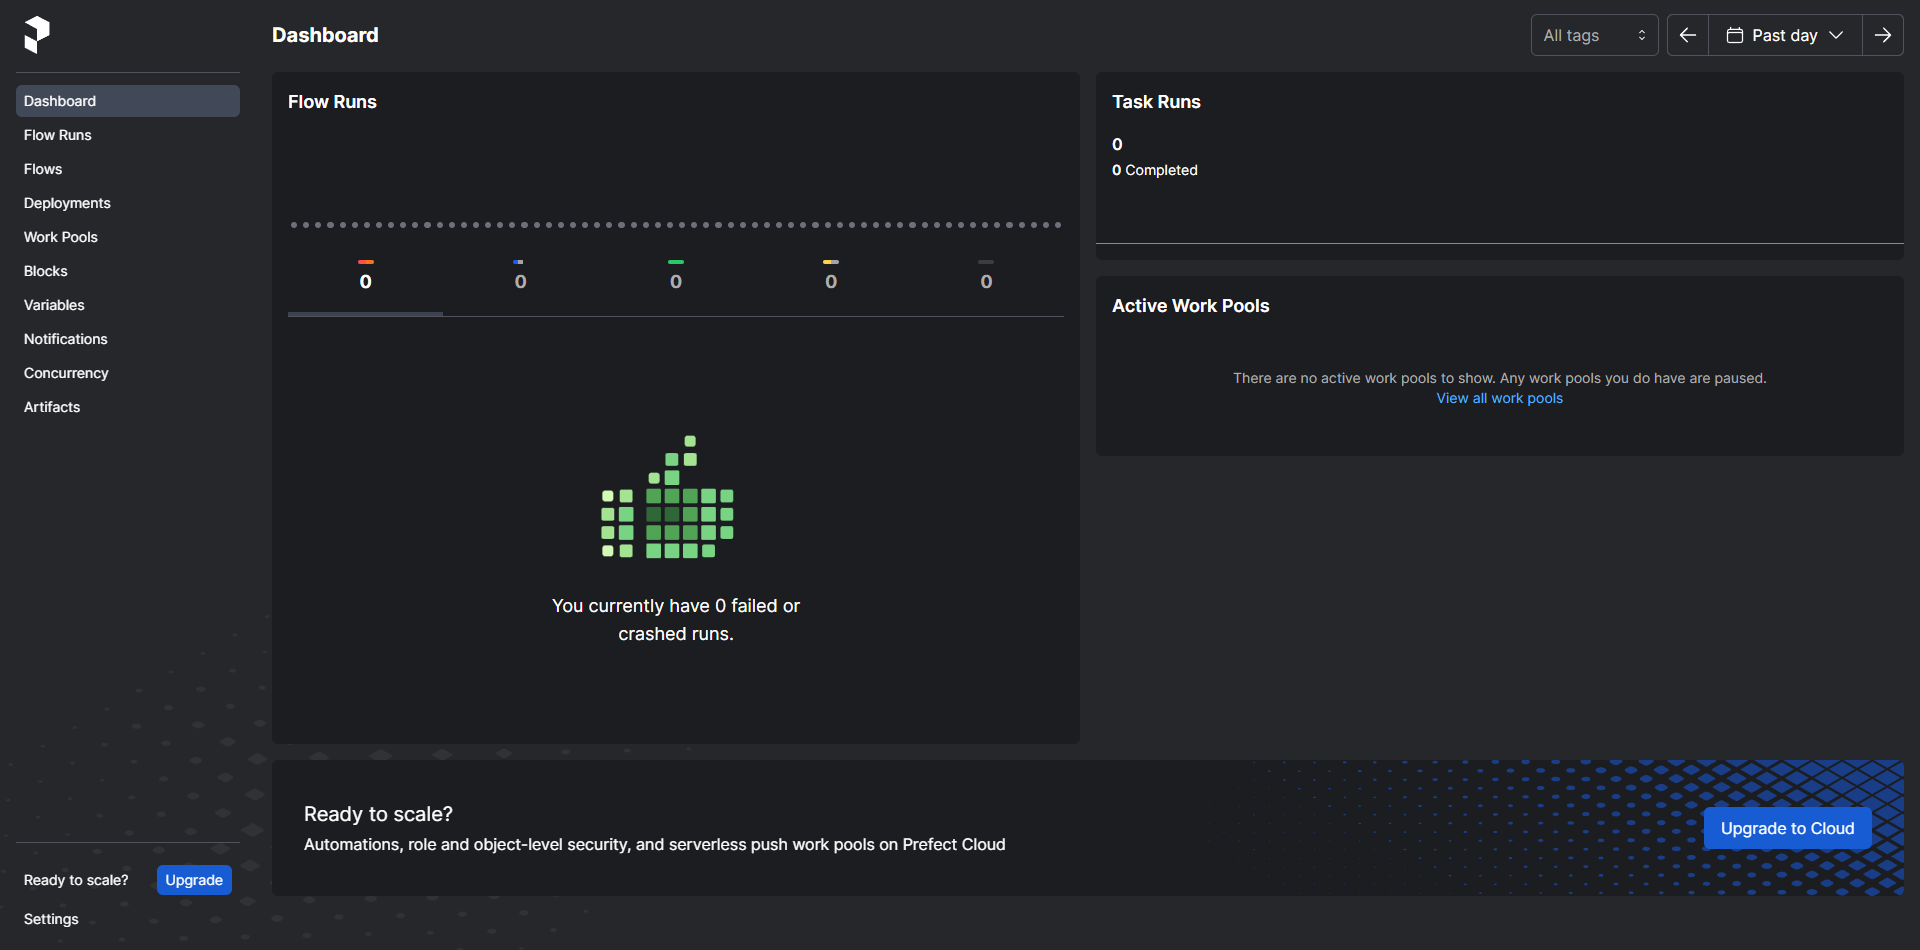
\includegraphics[width=\linewidth]{graphics/Prefect_dashboard.PNG}
    \caption{Prefect Dashboard}
    \label{fig:Prefect_Dashboard}
\end{figure}
De functies die kunnen worden gezien op figuur \ref{fig:Prefect_Dashboard} zijn:
\begin{itemize}
    \item \textbf{Dashboard:} Geeft een overzicht van alle flow runs, hier kan worden bekeken wanneer een flow succesvol of onsuccesvol is uitgevoerd.
    \item \textbf{Flow Runs:} Geeft een tijdlijn weer met alle flow die uitgevoerd zijn over een bepaalde tijd.
    \item \textbf{Flows:} Toont elke flow aan die in de code is geschreven. Hierbij kan ook in de flow gekeken worden om te zien welke taken het bevat.
    \item \textbf{Deployments:} Toont alle deployments weer, deze zijn flows die rechtstreeks met het dashboard kunnen worden uitgevoerd.
    \item \textbf{Blocks:} Hier worden alle gevoelige informatie bijgehouden, zoals wachtwoorden en API keys.
    \item \textbf{Work Pools:} Hier kan er verbinding gemaakt worden met een cloud omgeving om de pipeline daar te laten uitvoeren.
\end{itemize}
Dit Proof of Concept zal gebruik maken van de "Flow runs" en "Flows" pagina\'s op het dashboard.
\subsection{Uitvoering}
Prefect werkt met decorators, dit zorgt ervoor dat bestaande Python-functies makkelijk kunnen worden omgezet naar het Prefect framework. De twee decorators ``@task'' en ``@flow'' werden eerder in de stand van zaken uitgelegd. Deze maken het mogelijk om bestaande Python functies om te zetten naar het Prefect framework.

Origineel was preprocessing het downloaden en het verwerken van de afbeeldingen, maar voor het uitvoeren in Prefect is dit nog eens onderverdeeld geweest in twee aparte delen. Het downloaden en het verwerken gebeuren dus apart. Als bijlage kan de Prefect code te zien zijn.

De download functie werd een ``Task'' de andere functies werden een ``Flow''
Dit werd gedaan via de decorators voor de functie te plaatsen uiteindelijk worden dan alle ``Tasks'' en ``Flows'' samengevoegd in 1 pipeline.
\subsubsection{Pipeline}
De pipeline in Prefect is een flow waarin alle taken en flows achter elkaar worden uitgevoerd. De flow of pipeline ziet er als volgt uit:
\begin{minted}[frame=lines,breaklines,linenos]{python}
@flow(task_runner=SequentialTaskRunner(), log_prints=True)
def main():
    tracking_uri = "http://127.0.0.1:8080"
    model_name = "PoC"
    mlflow.set_tracking_uri(tracking_uri)
    mlflow.set_experiment(model_name)
    download()
    preprocess()
    model = train()
    eval(model)
\end{minted}

Deze code stelt eerst het juiste tracking adres in voor MLflow en de modelnaam. Hierna worden alle functies achter elkaar uitgevoerd en kunnen deze dan ook in de dashboard gezien worden zoals in figuur xxx.

In dit geval heeft de ``@flow'' nog extra parameters, deze betekenen:
\begin{itemize}
    \item task\_runner: Geeft aan hoe dat de taken en flows moeten uitgevoerd worden, in dit geval is dat een ``SequentialTaskRunner'' wat betekend dat alle tasks en flows achter elkaar worden uitgevoerd.
    \item log\_prints: Geeft alle prints weer dat in de Python code werd gebruikt, in dit geval is dat ``True'' dat maakt het gemakkelijk tijden het ontwikkelen van de pipeline.
\end{itemize}

Na het uitvoeren van de flow word deze flow gevisualiseerd in de web interface van Prefect. Figuur 
\subsection{Problemen}
Prefect had moeite met het doorgeven van parameters naar de volgende ``Task'', waardoor de flow niet meer kon werken. Om dit op te lossen is er gebruik gemaakt van een subflow. Subflows zijn flows die worden uitgevoerd in een bestaande flow. Deze ontvangen wel goed de parameters en kunnen alles goed uitvoeren.
\subsection{Cloud}
Prefect heeft een concept dat noemt ``Work Pools''. Figuur \ref{fig:Prefect_Work_Pools} toont hoe dat deze pagina in Prefect eruitziet:
\begin{figure}[htbp]
    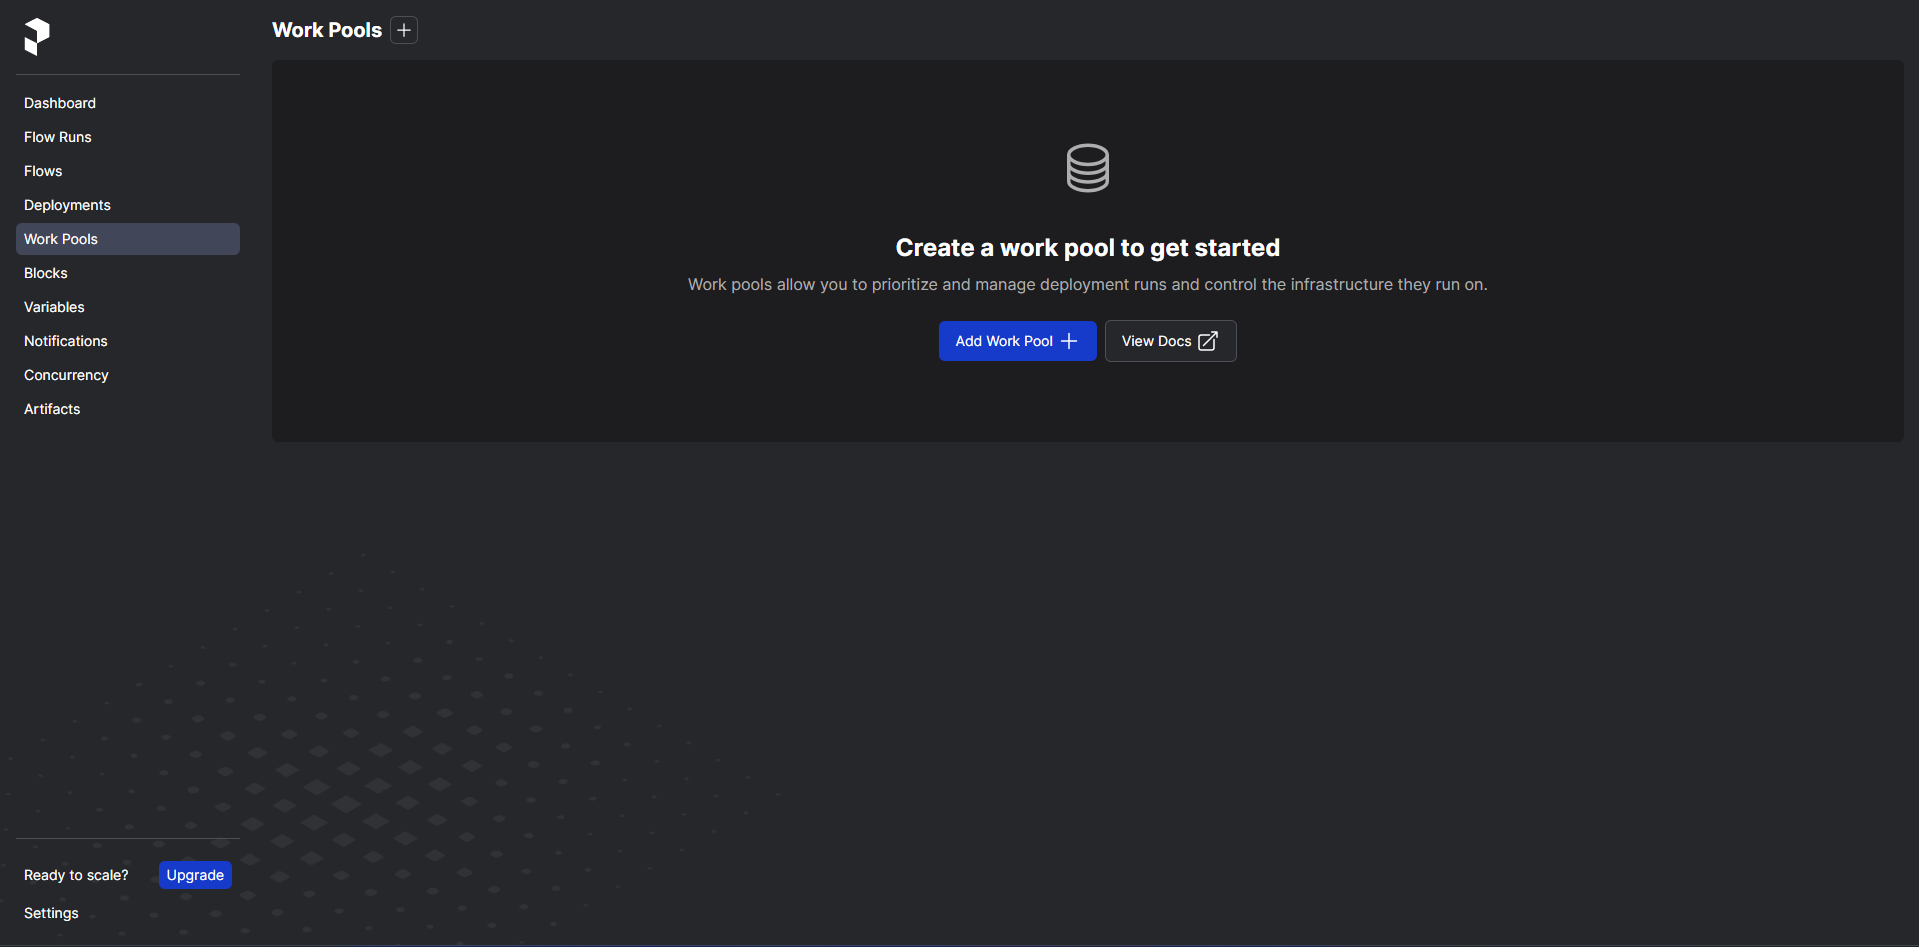
\includegraphics[width=\linewidth]{graphics/Prefect_Work_Pools.PNG}
    \caption{Prefect Work Pool Pagina}
    \label{fig:Prefect_Work_Pools}
\end{figure}
Op deze pagina kan er een ``Work Pool'' worden toegevoegd. Dit zorgt voor een verbinding met een cloud omgeving, zodat de Prefect flow in de cloud kan worden uitgevoerd. Het aanmaken van een verbinding kan via de knop ``Add Work Pool'' zoals te zien in figuur \ref{fig:Prefect_Work_Pools}.
Na het klikken van deze knop kan je kiezen met welke cloud omgeving dat er verbinding met gemaakt moet worden zoals te zien op figuur \ref{fig:Prefect_Work_Pools_Create}.
\begin{figure}[htbp]
    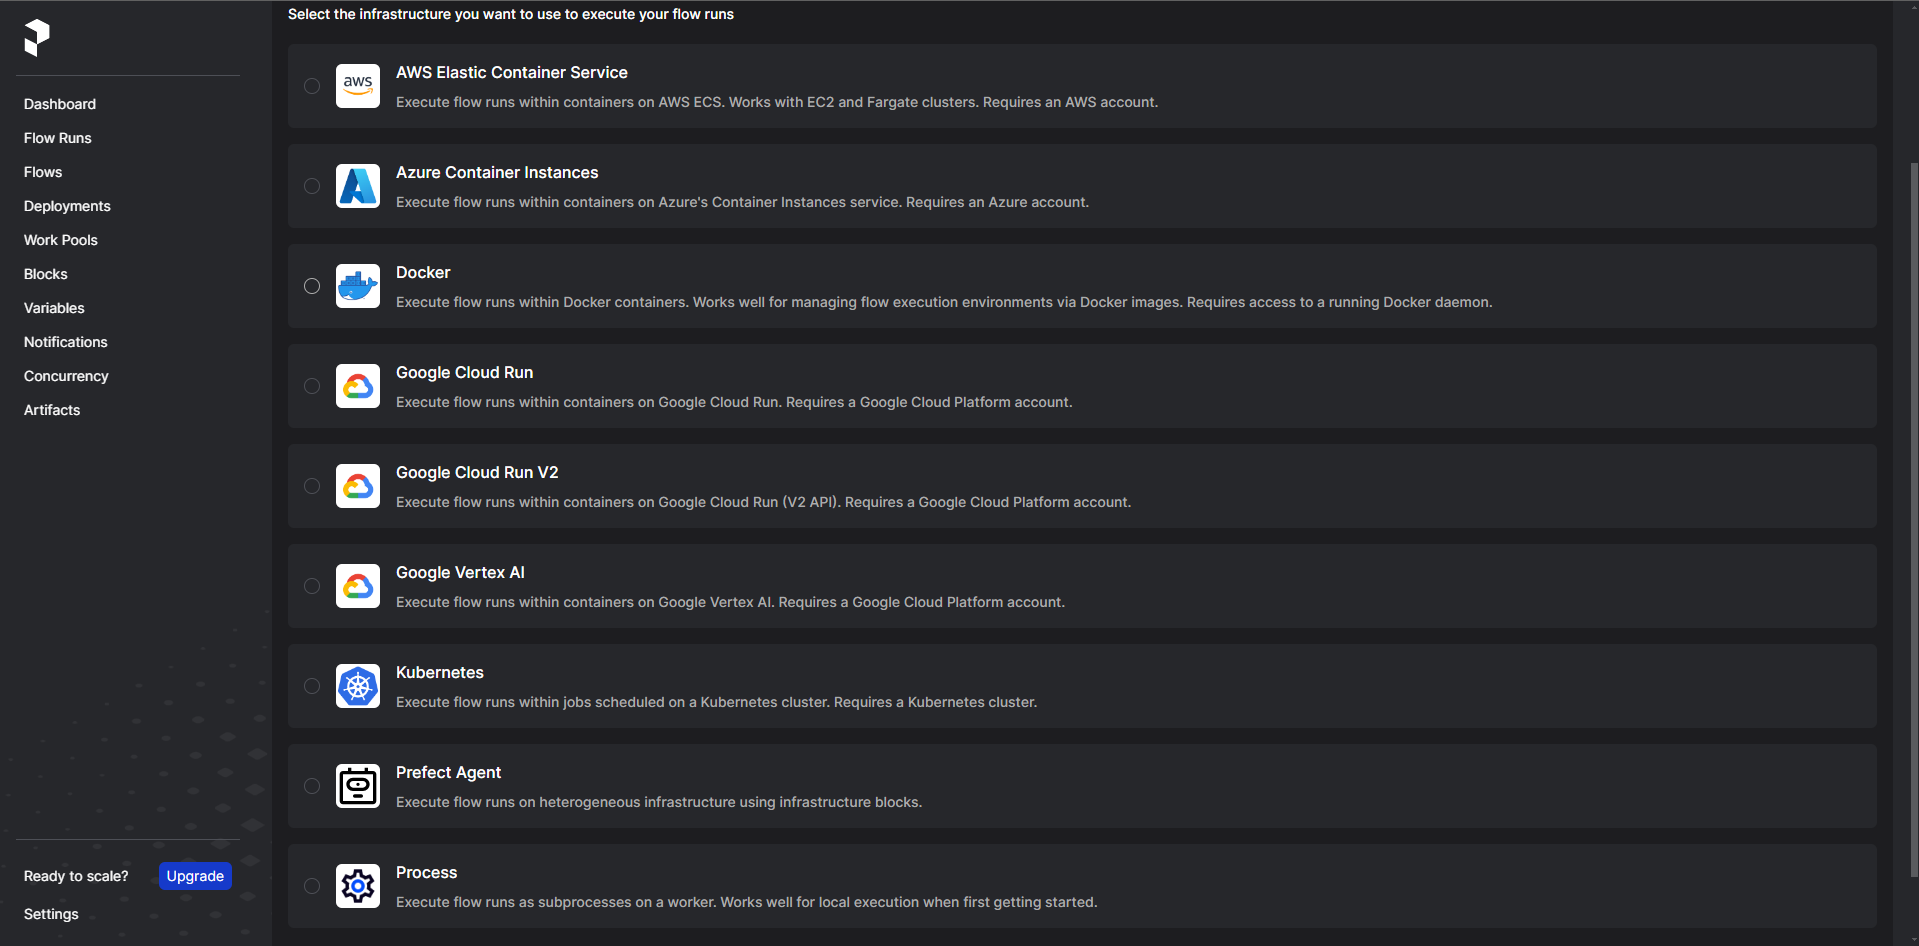
\includegraphics[width=\linewidth]{graphics/Prefect_Work_Pools_Create.PNG}
    \caption{Prefect Work Pool Cloud provider}
    \label{fig:Prefect_Work_Pools_Create}
\end{figure}
Figuur \ref{fig:Prefect_Work_Pools_Create} toont de verschillende cloud omgevingen waarmee Prefect kan werken. Deze omvatten onder andere:
\begin{itemize}
    \item AWS Elastic Container Service
    \item Azure Container Instances
    \item Docker
    \item Google Cloud Run
    \item Google Cloud Run v2
    \item Google Vertex AI
    \item Kubernetes
    \item Prefect Agent 
    \item Process
\end{itemize}
Voor dit voorbeeld selecteren we ``Process'' omdat er momenteel geen toegang is tot een cloudomgeving. De volgende stap is het invullen van details. Deze details zijn de naam en de beschrijving van de "Work Pool" en eventuele Concurrency. Alleen de naam is verplicht om in te vullen zoals te zien is in figuur \ref{fig:Prefect_Work_Pools_Create_Details}.
\begin{figure}[htbp]
    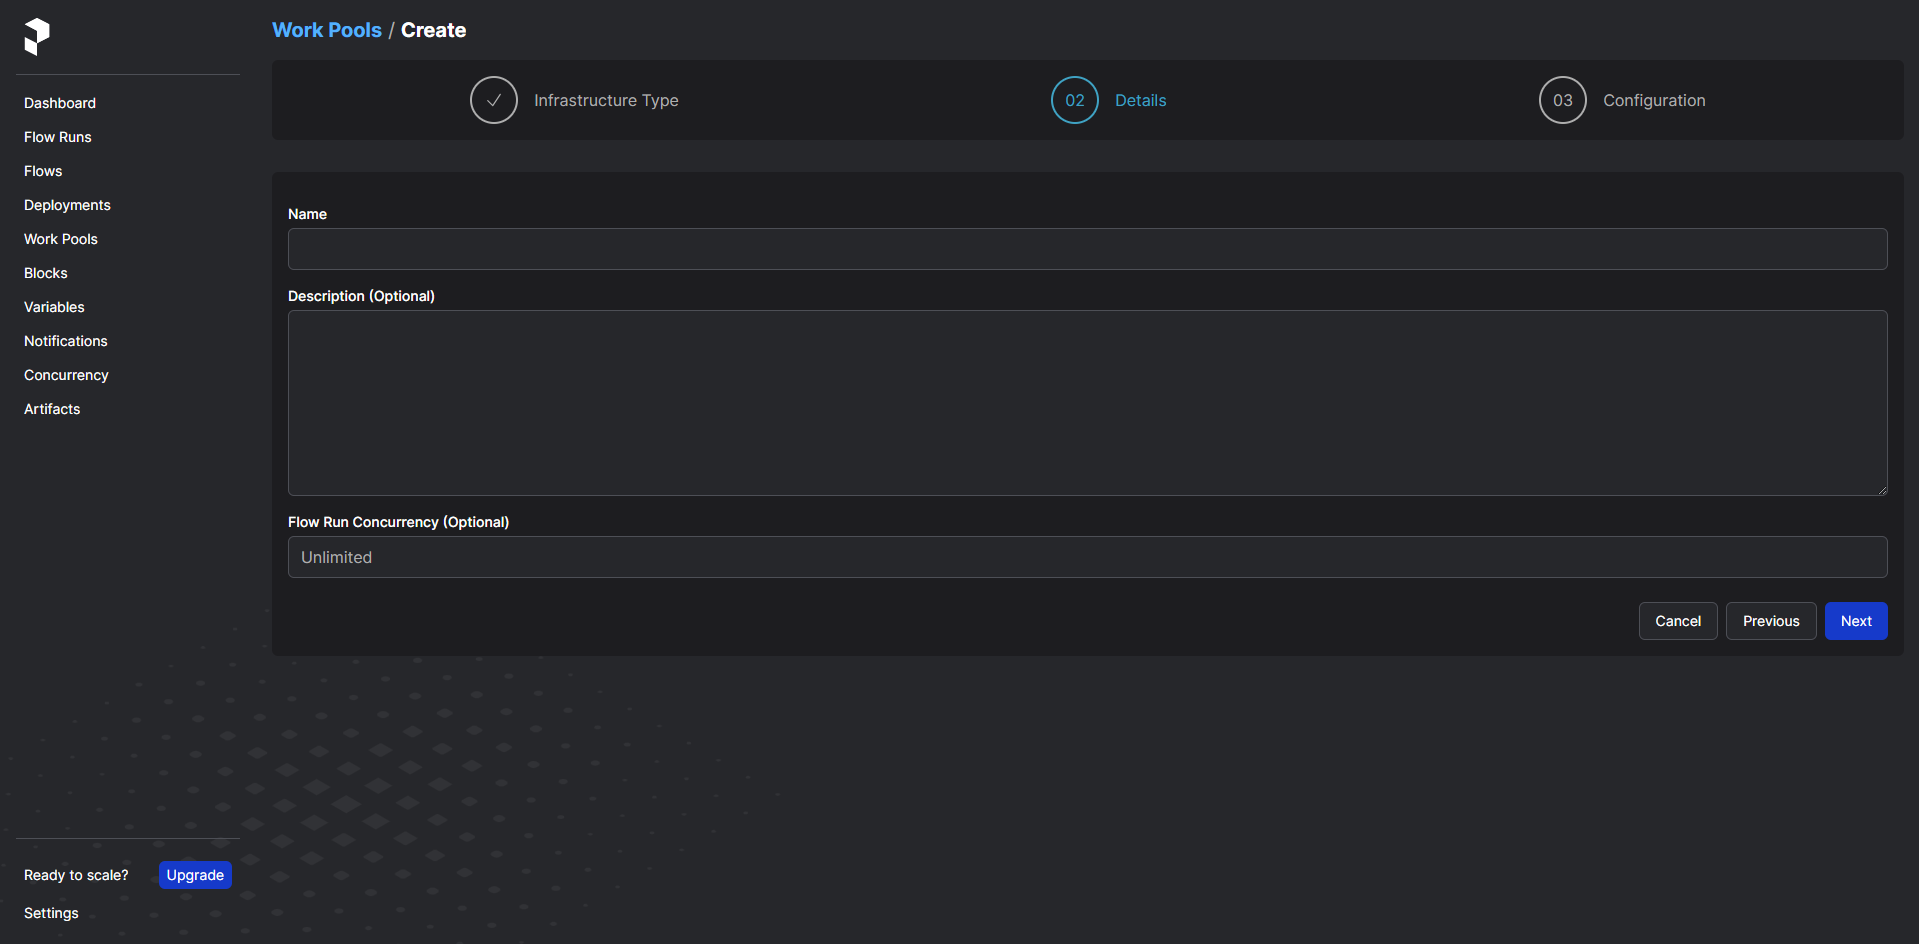
\includegraphics[width=\linewidth]{graphics/Prefect_Work_Pools_Create_Details.PNG}
    \caption{Prefect Work Pool Creation Details}
    \label{fig:Prefect_Work_Pools_Create_Details}
\end{figure}
Ten slotte, op de laatste pagina worden extra parameters ingesteld met betrekking tot de cloudprovider, zoals te zien is in figuur \ref{fig:Prefect_Work_Pools_Create_parameters}
\begin{figure}[htbp]
    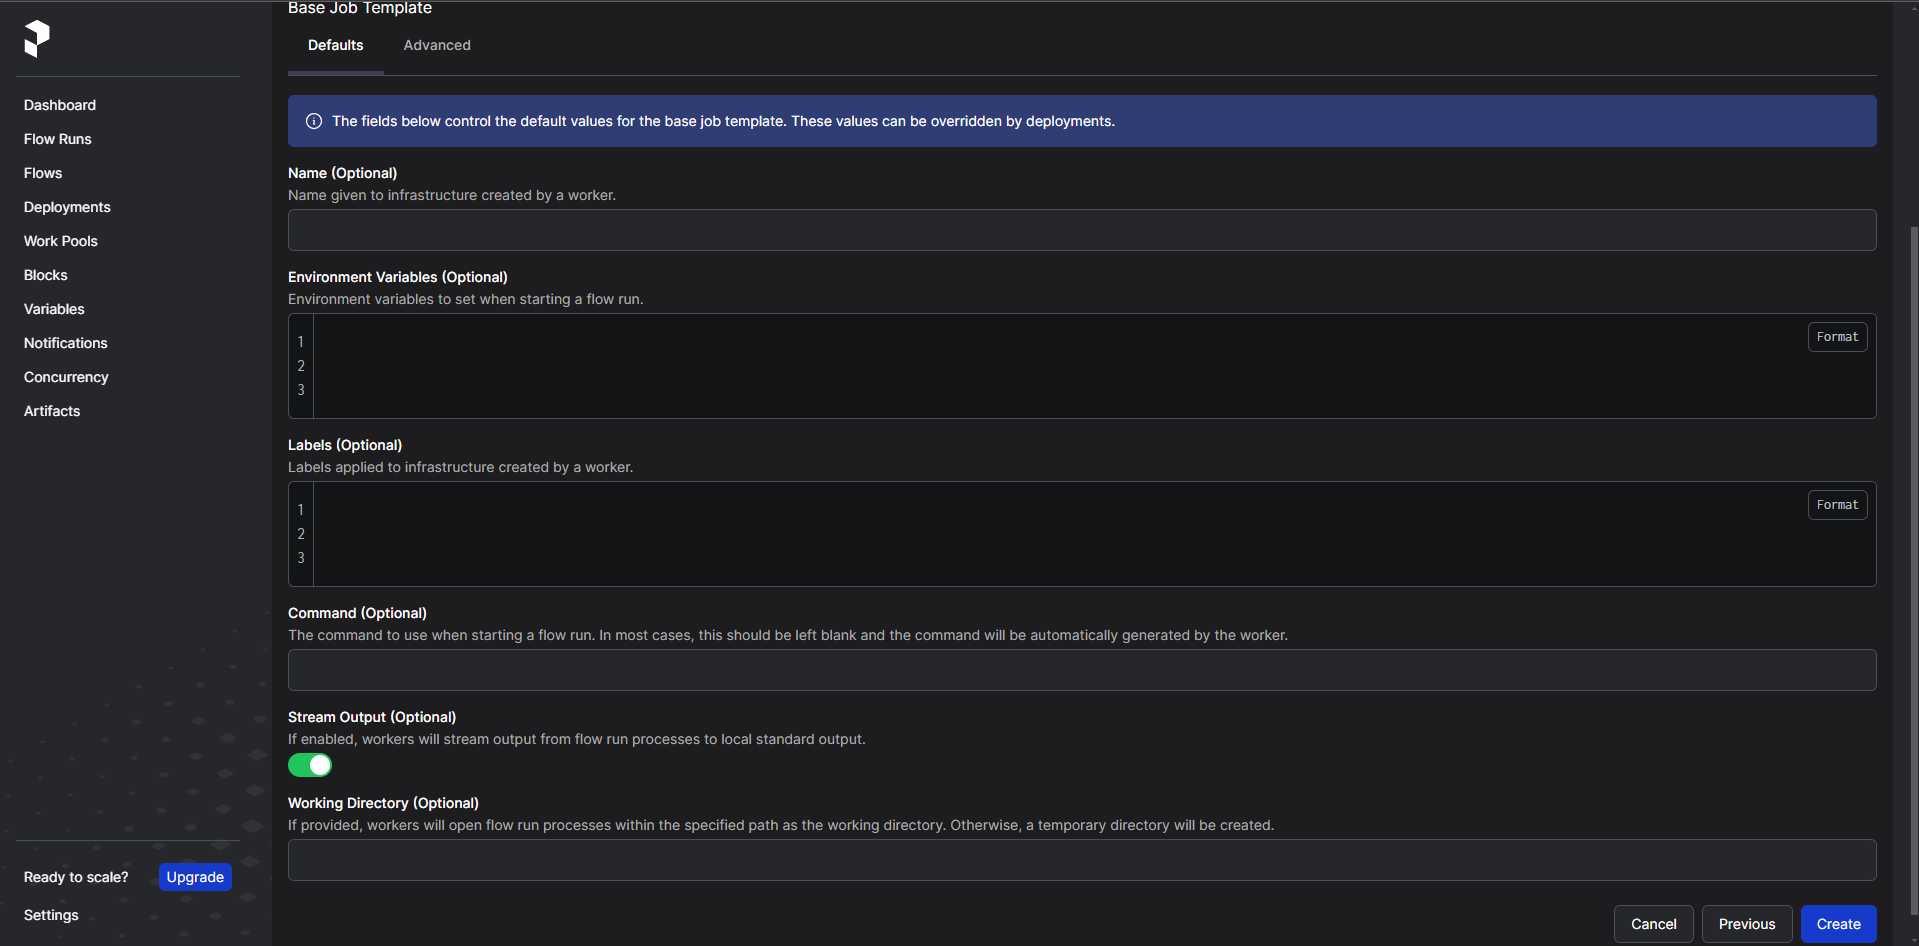
\includegraphics[width=\linewidth]{graphics/Prefect_Work_Pools_Create_Parameters.PNG}
    \caption{Prefect Work Pool Creation Details}
    \label{fig:Prefect_Work_Pools_Create_parameters}
\end{figure}
\section{ZenML}
\subsection{Installatie}
De installatie van ZenML is via de package manager ``pip'' en kan met het volgende commando geinstalleerd worden.
\begin{minted}[frame=lines,breaklines,linenos]{bash}
    pip install zenml
\end{minted}
Er moet wel rekening gehouden worden dat ZenML alleen werk met de Python versies 3.8, 3.9, 3.10 en 3.11.
Voor het lokaal uitvoeren van het ZenML dashboard moet er ook nog een extra package geinstalleerd worden:
\begin{minted}[frame=lines,breaklines,linenos]{bash}
    pip install "zenml[server]"
\end{minted}
\subsection{Dashboard}
\subsection{Uitvoering}
\subsection{Pipeline}
\subsection{Problemen}
\subsection{Cloud}
\section{Dagster}
\subsection{Installatie}
\subsection{Dashboard}
\subsection{Uitvoering}
\subsection{Pipeline}
\subsection{Problemen}
\subsection{Cloud}


